\documentclass[12pt]{article}

\usepackage{multicol}
\usepackage{textcomp}
\usepackage{amsmath,amssymb,amsfonts,latexsym,stmaryrd,graphicx}
\usepackage[utf8]{inputenc}
\usepackage[T1]{fontenc}
\usepackage{xcolor}
\usepackage{anyfontsize}
\usepackage[spanish]{babel}
\usepackage{listings}
\usepackage{latexsym}
\usepackage[pdftex,breaklinks,colorlinks,linkcolor=black,citecolor=black,urlcolor=black]{hyperref}

\usepackage{epstopdf}
\DeclareGraphicsExtensions{.pdf,.png,.jpg,.gif,.eps}

\newcommand{\proof}{\textbf{Demostración:} }
\newcommand{\nl}{\vspace{0.3cm}}

\newtheorem{theorem}{Teorema}
\newtheorem{lemma}{Lema}
\newtheorem{definition}{Definición}
\newtheorem{corollary}{Corolario}

%opening
\title{Proyecto de Diseño y Análisis de Algoritmos\\ \vspace{.2cm} \textbf{Algoritmo de Dijkstra}}
\author{Leynier Gutiérrez González}

\begin{document}

\maketitle

\vspace{0.5cm}

\begin{center}
	\vspace{0.2cm}
	
\includegraphics[width=2.5cm]{images/escudo.png}\\
	\vspace{0.2cm}
	Facultad de Matemática y Computación\\
	\vspace{0.1cm}
	Universidad de La Habana\\
	\vspace{1cm}
\end{center}

\vspace{1cm}

\begin{abstract}
	En este documento haremos una breve introducción al problema de los caminos de costo mínimo. Explicaremos y demostraremos el algoritmo de Dijkstra para la resolución de dicho problema y mostraremos varias aplicaciones del algoritmo para resolver ejercicios.
\end{abstract}

\newpage

\tableofcontents

\newpage

\section{Problema de los caminos más cortos}

\subsection{Definiciones}

\nl

Dados un grafo ponderado y dirigido $G = (V, E)$ y una función de peso $w: E \rightarrow \mathbb{R}$

\begin{definition}
	El peso de un camino $p = (v_1, v_2, ... , v_k)$ tal que $\forall i \ \ 1 \leqslant i \leqslant k; \ v_i \in V$; es la suma del peso de todas las aristas que lo constituyen:
	$$w(p) = \sum_{i=1}^{k} w(v_{i-1}, v_i)$$
\end{definition}

\begin{definition}
	El peso del camino más corto $\delta(u, v)$ desde el vértice $u$ hasta el vértice $v$ es:
	$$\delta(u, v) = \left\{ 
			\begin{array}{lcc}
				\min \{ w(p): u \stackrel{p}{\leadsto} v \} & si\; existe\; un\; camino\; desde\; u\; a\; v\; \\\\
				\infty & en\; caso\; contrario\;
			\end{array}
		\right. $$
\end{definition}

\begin{definition}
	Un camino más corto desde un vértice $u$ hasta un vértice $v$ se define como cualquier camino $p$ con peso $w(p) = \delta(u, v)$
\end{definition}

\subsection{Variantes del problema}

\nl

Existen varias variantes del problema de los caminos más cortos

\begin{itemize}
	\item Con una única fuente: Buscar el camino más corto desde un vértice fuente $s$ dado hasta todos los vértices $v \in V$. El algoritmo para una única fuente puede resolver muchos otros problemas, incluidas las siguientes variantes.
	\item Con un único destino: Buscar el camino más corto hasta un vértice destino $t$ dado desde todos los vértices $v \in V$. Al invertir la dirección de cada arista en el grafo, podemos reducir esta variante a la variante de una única fuente.
	\item Entre dos vértices: Buscar el camino más corto desde un vértice $u$ dado hasta un vértice $v$ dado. Si resolvemos esta variante del problema utilizando la variante de una única fuente con el vértice $u$ también estamos resolviendo el problema. Además, todos los algoritmos conocidos para esta variante del problema tienen el mismo tiempo de ejecución asintótico en el peor de los casos que los mejores algoritmos de la variante de una única fuente.
	\item Entre cualquier par de vértices: Buscar el camino más corto desde cualquier vértice $u \in V$ hasta cualquier vértice $v \in V$. Aunque podemos resolver este variante del problema ejecutando un algoritmo de fuente única una vez desde cada vértice, generalmente podemos resolverlo más rápido.
\end{itemize}

\subsection{Subestructura óptima de los caminos más cortos}

\nl

% Lemma 24.1 (Subpaths of shortest paths are shortest paths)
% Lema 1
\begin{lemma} Sea $p = (v_0, v_1, ... , v_k)$ un camino más corto desde el vértice $v_0$ hasta el vértice $v_k$, $\forall \;i, j$ tal que $0 \leqslant i \leqslant j \leqslant k$, y $p_{ij} = (v_i, v_{i+1}, ..., v_j)$ los subcaminos del camino $p$ desde el vértice $v_i$ hasta el vértice $v_j$. Entonces, $p_{ij}$ es un camino más corto desde $v_i$ hasta $v_j$.
\end{lemma}

\proof Si descomponemos el camino $p$ en $v_0 \stackrel{p_{0i}}{\leadsto} v_i \stackrel{p_{ij}}{\leadsto} v_j \stackrel{p_{jk}}{\leadsto} v_k$, entonces tenemos que $w(p) = w(p_{0i}) + w(p_{ij}) + w(p_{jk})$. Ahora, asumamos que existe el camino $p'_{ij}$ desde $v_i$ hasta $v_j$ con peso $w(p'_{ij}) < w(p_{ij})$. Entonces, $v_0 \stackrel{p_{0i}}{\leadsto} v_i \stackrel{p'_{ij}}{\leadsto} v_j \stackrel{p_{jk}}{\leadsto} v_k$ es un camino desde $v_0$ hasta $v_k$ con peso $w(p_{0i}) + w(p'_{ij}) + w(p_{jk})$ que es menor que $w(p)$ lo que contradice que $p$ sea un camino más corto luego queda demostrado que no existe un camino $p'_{ij}$ con menor peso que $p_{ij}$ entonces $p_{ij}$ es un camino más corto desde el vértice $v_i$ hasta el vértice $v_j$.

\subsection{Aristas con peso negativo}

Algunos casos del problema de los caminos más cortos desde una única fuente pueden incluir aristas con peso negativo.

\nl

Si el grafo no contiene ciclos con peso negativo alcanzables desde la fuente $s$, entonces $\forall \ v \in V$, los caminos con peso $\delta(s, v)$ permanecen bien definidos, incluso si es un valor negativo.

\nl

Por otro lado, si el grafo contiene ciclos con peso negativo alcanzables desde la fuente $s$, los pesos de los caminos más cortos no están bien definidos. Si existe un ciclo con peso negativo en algún camino desde $s$ a $v$, definimos el $\delta(s, v) = \infty$.

\subsection{Representación de los caminos más cortos}

\nl

Muy a menudos es necesario calcular el camino más corto y no sólo su peso. Esto se puede lograr manteniendo para cada vértice $v \in V$ un predecesor $v.p$ que es otro vértice o nulo. 

\nl

Los algoritmos para resolver el problema de los caminos más cortos mantienen los atributos $p$ para que las cadenas de predecesores que se originan desde un vértice $v$ representen los caminos más cortos desde $s$ a $v$.

\nl

Es importante mencionar que durante la ejecución de los algoritmos para resolver el problema de los caminos más cortos el valor de $p$ puede no indicar el camino más corto.

\begin{definition}
	Para el problema de los caminos más corto nos interesa en subgrafo de predecesores $G_p = (V_p, E_p)$ inducido por los valores de $p$ donde:
	$$ V_p = \{v \in V: v.p \neq nulo \} \cup \{s\} $$
	El conjunto de aristas dirigidas $E_p$ es el conjunto de aristas inducido por los valores de $p$ para los vértices de $V_p$:
	$$E_p = \{ (v.p, v) \in E: v \in V_p - \{ s \} \}$$
\end{definition}

\begin{definition}
	Sea $G = (V, E)$ un grafo dirigido y ponderado con una función de peso $w: E \rightarrow \mathbb{R} $ y asumimos que $G$ no contiene ciclos de peso negativo alcanzables desde el vértice fuente $s \in V$ para que los caminos más cortos estén bien definidos. Un árbol de caminos más cortos con raíz en $s$ es un subgrafo dirigido $G' = (V', E')$ donde $V' \subseteq V$ y $E' \subseteq E$ tal que:
	\begin{enumerate}
		\item $V'$ es el conjunto de vértices alcanzables desde $s$ en $G$.
		\item $G'$ forma un árbol con raíz en $s$.
		\item Para todo $v \in V$, el único camino simple desde $s$ a $v$ en $G'$ es un camino más corto desde $s$ a $v$ en $G$.
	\end{enumerate}
\end{definition}

Los caminos más cortos no son necesariamente únicos, y tampoco lo son los árboles de caminos más cortos.

\subsection{Inicialización y Relajación}

\nl

Muchos de los algoritmos para resolver el problema de los caminos más cortos utilizan una técnica llamada Relajación. Para cada vértice $v \in V$, mantienen un atributo $v.d$, que es una cota superior del peso del camino más corto desde la fuente $s$ hasta $v$.

\nl

El proceso de inicialización del los valores estimados de los caminos más cortos $v.d$ y los predecesores $v.p$ se realizara mediante el siguiente procedimiento cuya complejidad temporal es $O(|V|)$.

\nl

\textbf{Código 1} Proceso de inicialización

\lstinputlisting[language=Python]{codes/initialize_single_source.py}

\nl

El proceso de relajación de una arista $(u, v)$ consiste en probar si se puede mejorar el camino más corto hasta $v$ encontrado hasta el momento yendo a través de $u$, de ser así, actualizando $v.d$ y $v.p$. Un paso de relajación puede disminuir el valor de la estimación del peso del camino más corto $v.d$ y actualizar el predecesor $v.p$.

\nl

\textbf{Código 2} Proceso de relajación

\lstinputlisting[language=Python]{codes/relax.py}

\newpage

\subsection{Propiedades de los caminos más cortos}

\nl

El siguiente grupo de lemas describe como son afectados las estimaciones del peso de los caminos más cortos cuando se ejecutan una secuencia de relajaciones sobre las aristas de un grafo dirigido y ponderado luego del proceso de inicialización (\textbf{Código 1})

\subsubsection{Propiedad de la desigualdad triangular}

\nl

% Lemma 24.10 (Triangle inequality)
% Lema 2
\begin{lemma}
	Sea un grafo ponderado y dirigido $G = (V, E)$, una función de peso $w: E \rightarrow \mathbb{R}$ y un vértice fuente $s \in V$. Entonces, $\forall (u, v) \in E$ se cumple que:
	$$ \delta(s, v) \leqslant \delta(s, u) + w(u, v) $$
\end{lemma}

\proof Supongamos que $p$ es el camino más corto desde el vértice fuente $s$ hasta el vértice $v$. Entonces $p$ no tiene más peso que cualquier otro camino desde $s$ hasta $v$. Específicamente, el camino $p$ no tiene más peso que un camino particular que toma el camino más corto desde el vértice fuente $s$ hasta el vértice $u$ y luego toma la arista (u, v).

\subsubsection{Propiedad de la cota superior}

\nl

% Lemma 24.11 (Upper-bound property)
% Lema 3
\begin{lemma}
	Sea un grafo ponderado y dirigido $G = (V, E)$, una función de peso $w: E \rightarrow \mathbb{R}$, un vértice fuente $s \in V$, y el grafo fue inicializado con el \textbf{Código 1}. Entonces, $v.d \geqslant \delta(s, v) \; \forall v \in V$, y esta invariante es mantenida sobre cualquier secuencia de pasos de relajación sobre las aristas de $G$. Además, una vez que $v.d$ alcanza su cota inferior $\delta(s, v)$, nunca cambia.
\end{lemma}

\proof Probaremos que la invariante $v.d \geqslant \delta(s, v) \; \forall v \in V$ por inducción en el número de pasos de relajación.

\nl

Para el caso base, $v.d \geqslant \delta(s, v)$ es verdadero después de la inicialización, ya que $v.d = \infty$ implica que $v.d \geqslant \delta(s, v) \; \forall v \in V - \{ s \}$, y ya que $s.d = 0 \geqslant \delta(s, s)$ (notar que $\delta(s, s) = -\infty$ si $s$ está en un ciclo de aristas con peso negativo y $0$ en caso contrario).

\nl

Para el paso inductivo, consideremos la relajación de la arista $(u, v)$. Por hipótesis de inducción, $x.d \geqslant \delta(s, x) \; \forall x \in V$ antes de la relajación. El único valor $d$ que puede cambiar es el del $v.d$. Si cambia, tenemos:
\begin{eqnarray*}
	v.d	& =       	& u.d + w(u, v) \\
	& \geqslant	& \delta(s, u) + w(u, v) \ (por\ hipotesis\ de\ induccion) \\
	& \geqslant	& \delta(s, v) \ (por\ el\ Lema\ 2)
\end{eqnarray*}

y por tanto, la invariante es mantenida.

\nl

Para ver que el valor de $v.d$ nunca cambia después que $v.d = \delta(s, v)$, hay que notar que ha alcanzado si cota inferior, $v.d$ no pude disminuir porque $v.d \geqslant \delta(s, v)$, y este no puede aumentar porque los pasos de relajación no aumentan los valores de $d$.

% Corollary 24.12 (No-path property)
% Corolario 1
\begin{corollary}
	Supongamos que en un grafo ponderado y dirigido $G = (V, E)$ con una función de peso $w: E \rightarrow \mathbb{R}$ tal que no existe ningún camino desde el vértice fuente $s \in V$ a un vértice dado $v \in V$. Entonces, luego de inicializar el grafo con el \textbf{Código 1}, se cumplirá que $v.d = \delta(s,v) = \infty$, y esta igualdad se mantendrá como una invariante sobre cualquier secuencia de paso de relajación sobre las aristas de $G$.
\end{corollary}

\proof Por el \textbf{Lema 3}, tenemos siempre $\infty = \delta(s, v) \leqslant v.d$, y así $v.d = \infty = \delta(s, v)$.

% Lemma 24.13
% Lema 4
\begin{lemma}
	Sea un grafo ponderado y dirigido $G = (V, E)$, una función de peso $w: E \rightarrow \mathbb{R}$ y una arista $(u, v) \in E$. Entonces, inmediatamente después de relajar la arista $(u, v)$ por la ejecución del \textbf{Código 2}, se cumplirá que $v.d \leqslant u.d + w(u, v)$.
\end{lemma}

\proof Si, justo antes de relajar la arista $(u, v)$, tenemos que $v.d > u.d + w(u, v)$, entonces después de la relajación $v.d = u.d + w(u, v)$. Si, al contrario, $v.d \leqslant u.d + w(u, v)$ justo antes de la relajación, entonces ni $u.d$ ni $v.d$ cambian, y por lo tanto después de la relajación $v.d \leqslant u.d + w(u, v)$.

\subsubsection{Propiedad de la convergencia}

\nl

% Lemma 24.14 (Convergence property)
% Lema 5
\begin{lemma}
	Sea un grafo ponderado y dirigido $G = (V, E)$, una función de peso $w: E \rightarrow \mathbb{R}$, un vértice fuente $s \in V$, y un camino más corto $s \leadsto u \rightarrow v $ en $G$ para algunos vértices $u, v \in V$. Suponiendo que el grafo $G$ fue inicializado por el \textbf{Código 1} y luego una secuencia de pasos de relajación con las llamadas al \textbf{Código 2} sobre las aristas de $G$. Si $u.d = \delta(s, u)$ antes de la llamada, entonces será en todo momento $v.d = \delta(s, v)$ después de la llamada.
\end{lemma}

\proof Por el \textbf{Lema 3}, si $u.d = \delta(s, u)$ en algún punto antes de la relajación de la arista $(u, v)$, entonces esta igualdad se mantiene a partir de entonces. En particular después de relajar, tenemos que:
\begin{eqnarray*}
	v.d	& \leqslant	& u.d + w(u, v) \ (por\ el\ Lema\ 3) \\
	& =			& \delta(s, u) + w(u, v) \\
	& =			& \delta(s, v) \ (por\ el\ Lema\ 1)
\end{eqnarray*}

Por el \textbf{Lema 3}, $v.d \geqslant \delta(s, v)$, de aquí concluimos que $v.d = \delta(s, v)$, y esta igualdad se mantiene a partir de entonces.

\subsubsection{Propiedad de la relajación de un camino}

\nl

% Lemma 24.15 (Path-relaxation property)
% Lema 6
\begin{lemma}
	Sea un grafo ponderado y dirigido $G = (V, E)$ con función de peso $w: E \rightarrow \mathbb{R}$, y sea $s \in V$ un vértice fuente. Considerando cualquier camino más corto $p = (v_0, v_1, ..., v_k)$ de $s = v_0$ a $v_k$. Si $G$ se inicializa con el \textbf{Código 1} y luego se realiza una secuencia de pasos de relajación que incluye, en orden, relajar las aristas $(v_0, v_1), (v_1, v_2), ..., (v_{k-1}, v_k)$, luego $v_{k}.d = \delta(s, v_k)$ después de estas relajaciones y en todo momento después. Esta propiedad se mantiene sin importar lo que ocurra con otras relajaciones de aristas, incluidas las relajaciones que se entremezclan con las relajaciones de las aristas de $p$.
\end{lemma}

\proof Demostraremos por inducción que después que la i-esima arista del camino $p$ fue relajada, se cumple que $v_{i}.d = \delta(s, v_i)$.

\nl

Para el caso base $i = 0$ y antes de que cualquier arista de $p$ haya sido relajada, tenemos por la inicialización que $v_{0}.d = s.d = 0 = \delta(s, s)$. Por el \textbf{Lema 3}, el valor de $s.d$ nunca cambiará después de la inicialización.

\nl

Para el paso inductivo, asumiremos que $v_{i-1}.d = \delta(s, v_{i-1})$, y vamos a ver que pasa cuando relajemos la arista $(v_{i-1}, v_i)$. Por el \textbf{Lema 5}, después de relajar esta arista, tenemos que $v_{i}.d = \delta(s, v_i)$, y esta igualdad se mantiene en todo momento a partir de entonces.

\nl

En los siguientes lemas mostramos que una vez que una secuencia de relajaciones ha hecho que las estimaciones del camino más corto converjan a al peso del camino más corto, el subgrafo predecesor $G_p$ inducido por los valores de $p$ resultantes es un árbol de caminos más cortos para $G$.

% Lemma 24.16
% Lema 7
\begin{lemma}
	Sea un grafo ponderado y dirigido $G = (V, E)$ con función de peso $w: E \rightarrow \mathbb{R}$, sea $s \in V$ un vértice fuente y supongamos que $G$ no contiene ciclos de peso negativos que sean accesibles desde $s$. Luego, una vez que el grafo se inicializa con el \textbf{Código 1}, el subgrafo predecesor $G_p$ forma un árbol con raíz $s$, y cualquier secuencia de pasos de relajación en las aristas de $G$ mantiene esta propiedad como invariante.
\end{lemma}

\proof Inicialmente, el único vértice en $G_p$ es el vértice fuente $s$, el lema es verdadero. Consideremos un subgrafo de predecesores $G_p$ que surge después de una secuencia de pasos de relajación. Probaremos primero que el grafo $G_p$ es acíclico. Suponiendo para llegar a una contradicción que algún paso de relajación creó un ciclo en $G_p$. Sea $c = (v_0, v_1, ..., v_k)$ el ciclo, donde $v_k = v_0$. Entonces, $v_{i}.p = v_{i-1}$ para $i = 1, 2, ..., k$ y, sin pérdida de generalidad, asumiremos que el paso de relajación que creó en ciclo fue sobre la arista $(v_{k-1}, v_k)$.

\nl

Todos los vértices del ciclo $c$ son alcanzables desde $s$ porque cada vértice en $c$ tiene un predecesor, y a cada vértice de $c$ fue asignado con una estimación del peso del camino más corto finito cuando fue asignado su predecesor diferente de nulo. Por el \textbf{Lema 3}, cada vértice del ciclo $c$ tiene un peso finito del camino más corto lo que implica que todos sean alcanzables desde $s$.

\nl

Examinaremos las estimaciones del peso del camino más corto de los vértices de $c$ justo antes de la ejecución del paso de relajación sobre la arista $v_{k-1}, v_k$ y mostraremos que $c$ es un ciclo de peso negativo, creando una contradicción con lo asumido de que $G$ no contiene ciclos de peso negativo alcanzables desde $s$. Justo antes de la ejecución, tenemos que $v_{i}.p = v_{i-1}$ para $i = 1, 2, ..., k - 1$. Así, para $i = 1, 2, ..., k - 1$, la última actualización de $v.d$ fue por la asignación $v_{i}.d = v_{i-1}.d + w(v_{i-1}, v_{i})$. Si $v_{i-1}.d$ cambió, entonces decreció. Por lo tanto, justo antes de la relajación tenemos que:

$$ v_{i}.d \geqslant v_{i-1}.d + w(v_{i-1}, v_i) \ \forall i = 1, 2, ..., k-1$$

Porque $v_{p}.k$ fue cambiado por la relajación, inmediatamente antes teníamos que:

$$ v_{k}.d > v_{k-1}.d + w(v_{k-1}, v_k)$$

Sumando $k-1$ veces la desigualdad anterior obtenemos la suma de los pesos estimados del camino más corto del ciclo $c$.

\begin{eqnarray*}
	\sum_{i=1}^{k} v_{i}.d 	& > & \sum_{i=1}^{k}(v_{i-1}.d + w(v_{i-1}, v_i)) \\
	& = & \sum_{i=1}^{k} v_{i-1}.d + \sum_{i=1}^{k} w(v_{i-1},v_i)
\end{eqnarray*}

Pero

$$ \sum_{i=1}^{k} v_{i}.d = \sum_{i=1}^{k} v_{i-1}.d $$

Ya que cada vértice en el ciclo $c$ aparece exactamente una vez en cada suma. Esta igualdad implica que

$$ 0 > \sum_{i=1}^{k} w(v_{i-1},v_i) $$

Ya que, la suma de los pesos del ciclo $c$ es negativa, llegamos a la contradicción deseada.

\nl

Ahora, probaremos que $G_p$ es un grafo dirigido y acíclico. Para demostrar que es un árbol con $s$ como raíz, es suficiente probar que para cada vértice $v \in V_p$ existe un único camino simple desde $s$ a $v$ en $G_p$.

\nl

Primero, debemos demostrar que el camino desde $s$ existe para cada vértice que pertenece a $V_p$. Los vértices de $V_p$ son aquellos con los valores $p$ no nulos más $s$. La idea aquí es probar por inducción que existe un camino desde $s$ a todos los vértices en $V_p$.

\nl

Para completar la demostración del lema, demostraremos que para cualquier vértice $v \in V_p$, el grafo $G_p$ contiene a lo sumo un camino simple desde $s$ a $v$. Supongamos lo contrario, que $G_p$ contiene dos caminos simples desde $s$ a $v$. Sean $p_1 = s \rightsquigarrow u \rightsquigarrow y \rightarrow z \rightsquigarrow v $ y $p_2 = s \rightsquigarrow u \rightsquigarrow x \rightarrow z \rightsquigarrow v $ donde $x \neq y$ (aunque $u$ podría ser $s$ y $z$ podría ser $v$). Pero entonces, $z.p = x$ y $z.p = y$ lo que implica la contradicción de que $x = y$. Llegamos a la conclusión de que $G_p$ contiene un único camino simple de $s$ a $v$, y por lo tanto, $G_p$ forma un árbol con raíz $s$.

\nl

Luego si, después de haber realizado una secuencia de pasos de relajación, a todos los vértices se les han asignado sus verdaderos pesos de los caminos más cortos, entonces el subgrafo $G_p$ de predecesores es un árbol de caminos más cortos.

\subsubsection{Propiedad del subgrafo de predecesores}

% Lemma 24.17 (Predecessor-subgraph property)
% Lema 8
\begin{lemma}
	Sea un grafo ponderado y dirigido $G = (V, E)$ con función de peso $w: E \rightarrow \mathbb{R}$, sea $s \in V$ un vértice fuente y supongamos que $G$ no contiene ciclos de peso negativos que sean accesibles desde $s$. El grafo se inicializó con el \textbf{Código 1} y luego se aplicó cualquier secuencia de pasos de relajación en las aristas de $G$ que produjo que $v_d = \delta(s, v) \; \forall v \in V$. Luego, el subgrafo predecesor $G_p$ es un árbol de caminos más cortos con $s$ como raíz.
\end{lemma}

\proof Debemos probar que las tres propiedades de los árboles de caminos más cortos que figuran en la \textbf{Definición 5} se mantienen para $G_p$. Para demostrar la primera propiedad, debemos demostrar que $V_p$ es el conjunto de vértices alcanzables desde $s$. Por definición, el peso de camino más corto $\delta(s, v)$ es finito si y sólo si $v$ es alcanzable desde $s$, y por lo tanto los vértices que son alcanzables desde $s$ son exactamente aquellos con valores $d$ finitos. Pero a un vértice $v$ se le ha asignado un valor finito para $v.d$ si y sólo si $v.p$ no es nulo. Por lo tanto, los vértices en $V_p$ son exactamente los alcanzables desde $s$.

\nl

La segunda propiedad se demuestra directamente de \textbf{Lema 7}.

\nl

Queda, por tanto, probar la última propiedad de los árboles de caminos más cortos: para cada vértice $v \in V_p$, el único camino simple $ s \stackrel{p}{\rightsquigarrow} v $ in $G_p$ es un camino más corto desde $s$ a $v$ en $G$. Sea $p = (v_0, v_1, ..., v_k)$, donde $v_0 = s$ y $v_k = v$. Para $i = 1, 2, ..., k$ tenemos que $v_{i}.d = \delta(s, v_i)$ y $v_{i}.d \geqslant v_{i-1}.d + w(v_{i-1}, v_i)$, de aquí concluimos que $w(v_{i-1}, v_i) \leqslant \delta(s, v_i) - \delta(s, v_{i-1})$. Sumando los pesos a lo largo del camino p

\begin{eqnarray*}
	w(p) & = & \sum_{i=1}^{k} w(v_{i-1}, v_i) \\
	& \leqslant & \sum_{i=1}^{k} (\delta(s, v_i) - \delta(s, v_{i-1})) \\
	& = & \delta(s, v_k) - \delta(s, v_0) \\
	& = & \delta(s, v_k)
\end{eqnarray*}

Así, $w(p) \leqslant \delta(s, v_k)$. Ya que $\delta(s, v_k)$ es una cota mínima para el peso de cualquier camino desde $s$ a $v$, concluimos que $w(p) = \delta(s, v_k)$, y por lo tanto $p$ es el camino más corto desde $s$ hasta $v_k$.

\section{Algoritmo de Dijkstra}

\subsection{Explicación}

\nl

El algoritmo de Dijkstra resuelve el problema de los caminos más cortos en un grafo $G = (V, E)$ dirigido y ponderado para el caso en que todas las aristas sean de peso no negativos. El algoritmo mantiene un conjunto de vértices $S$ donde el peso del camino más corto desde el vértice fuente $s$ ya está calculado. El algoritmo repetidamente selecciona el vértice $u \in V - \{s\}$ con el menor peso estimado del camino más corto. Añade $u$ a $S$ y relaja todas las aristas que salen de $u$.

\nl

En la siguiente implementación se utiliza una cola con prioridad de mínimos Q para los vértices cuyas llaves son los valores $d$.

\newpage

\textbf{Código 1} Proceso de inicialización

\lstinputlisting[language=Python]{codes/dijkstra.py}

\nl

Esta es la implementación clásica, más adelante veremos otra implementación ligeramente diferente y totalmente funcional en Python 3.

\nl

La línea 2 inicializa los valores de $d$ y $p$ de la manera usual y en la línea 3 inicializa el conjunto $S$ vacío. El algoritmo mantiene el invariante de $Q = V - S$ al comienzo de cada iteración del ciclo $while$ de las líneas 5 a 9. En la línea 4 inicializa la cola con prioridad $Q$ conteniendo todos los vértices de $V$, ya que $S = \emptyset$ en ese momento, entonces la invariante es verdadera en la línea 4. Cada iteración del ciclo en la línea 6 se extrae un vértice $v$ de $Q$ y en la línea 7 se añade al conjunto $S$, provocando que se mantenga la invariante. El vértice $u$, por lo tanto, tiene la menor estimación del peso de camino más corto de cualquier vértice en $V - S$. Entonces, las líneas 8-9 relajan las aristas que salen del vértice $u$, actualizando así la estimación del peso $v.d$ y el predecesor $v.p$ si se puede mejorar el camino más corto hasta $v$ encontrado hasta el momento mediante la arista $(u, v)$.

\nl

Observe que el algoritmo nunca inserta vértices en Q después de la línea 4 y que cada vértice se extrae de Q y se agrega a S exactamente una vez, de modo que el ciclo $while$ de las líneas 5–9 se hace exactamente $|V|$ veces.

\subsection{Correctitud}

\begin{theorem}
	El algoritmo de Dijkstra ejecutado sobre un grafo $G = (V,E) $ dirigido y ponderado, con una función no negativa $w$ y una fuente $s$, termina con $u.d = \delta(s, u) \; \forall u \in V$.
\end{theorem}

\proof Probaremos que al comienzo de cada iteración del ciclo $while$ de las líneas $5-9$, $v.d = \delta(s, v) \; v \in S$.

\nl

Es suficiente demostrar que $\forall \; u \in V$ en el momento en que $u$ es añadido al conjunto $S$, $u.d = \delta(s, u)$. Una vez que demostremos lo anterior, nos apoyaremos en el Lema 3 que plantea que la igualdad $u.d = \delta(s, u)$ se mantendrá durante la ejecución del programa.

\nl

Inicialmente $S = \emptyset$ y por tanto la invariante se cumple. Demostraremos que en cada iteración, $u.d = \delta(s,u)$ para el vértice $u$ agregado al conjunto $S$. Para lograr una contradicción, sea $u$ el primer vértice con $u.d \neq \delta(s,u)$ cuando este es añadido a $S$.

\nl

Centraremos nuestra atención en la situación al comienzo de la iteración del ciclo $while$ en el que $u$ se agrega a $S$ y daremos pie a una contradicción de que $u.d = \delta(s, u)$ en ese momento buscando un camino más corto de $s$ a $u$. Debemos tener que $u \neq s$ porque $s$ es el primer vértice añadido a $S$ y $s.d = \delta(s, s) = 0$ en ese momento. Debido a que $u \neq s$ tenemos que $S \neq \emptyset$ justo antes de añadir $u$ a $S$. Tenemos que debe existir un camino desde $s$ a $u$, de otra manera $u.d = \delta(s, u) = \infty$ por el Corolario 1, lo que violaría nuestra suposición de que $u.d \neq \delta(s, u)$. Como hay al menos existe un camino, entonces existe un camino más corto $p$ entre $s$ y $u$.

\nl

Antes de añadir $u$ a $S$, el camino $p$ que conecta los vértices en $S$, es decir $s$, a los vértices de $V - S$ es decir $u$. Consideremos el primer vértice $y$ en $p$ tal que $y \in V - S$, sea $x \in S$ el predecesor de $y$ en el camino $p$. Ya que, se puede descomponer el camino $p$ en $ s \stackrel{p_1}{\rightsquigarrow} x \rightarrow y \stackrel{p_2}{\rightsquigarrow} u $ (cualquiera de las rutas $p_1$ o $p_2$ puede no tener aristas). Podemos afirmar que $ y.d = \delta(s, y) $ cuando $u$ es añadido a $S$. Para esto demostraremos que $x \in S$, por tanto, como asumimos que $u$ es el primer vértice para el cual $u.d \neq \delta(s, u)$, cuando dicho vértice se adiciona a $S$, se tenía que $x,d = \delta(s, x)$. Cuando $x$ se insertó en $S$, la arista $(x, y)$ y en ese momento se hizo $y.d = \delta(s, y)$ por el Lema 5.

\newpage

A partir de lo anterior lleguemos a la contradicción para probar que $u.d = \delta(s, u)$. Como $y$ esta antes que $u$ en $p$ (camino más corto desde $s$ a $u$) donde todos las aristas tienen pesos no negativos, entonces, $\delta(s, y) < \delta(s, u)$ y por lo tanto:

\begin{eqnarray*}
	y.d & = & \delta(s, y) \\
	& \leqslant & \delta(s, u) \\
	& \leqslant & u.d \ (por\ el\ Lema\ 3)
\end{eqnarray*}

Como $u$ y $y$ estaban en $V - S$ en el momento en que $u$ fue seleccionado en la línea 6, entonces,  $u.d \leqslant y.d$ y teniendo en cuenta la desigualdad $y.d \leqslant \delta(s, u)$ tenemos que:

$$ y.d = \delta(s, y) = \delta(s, u) = u.d $$

En consecuencia, $u.d = \delta(s, u)$, que contradice nuestra elección de $u$. Concluimos que $u.d = \delta(s, u)$ cuando se agrega $u$ a S, y que esta igualdad se mantiene en todo momento posterior.

\nl

Al terminar el algoritmo, $Q = \emptyset$ lo cual, a partir de nuestra invariante de que siempre $Q = V - S$, implica $S = V$, por tanto, $u.d = \delta(s, u) \ \forall u \in V$.

\begin{corollary}
	Si ejecutamos el algoritmo de Dijkstra en un grafo $G = (V,E) $ dirigido ponderado con función de peso no negativa $w$ y un vértice fuente $s$, luego en la terminación, el subgrafo $G$ predecesor es un árbol de caminos más cortos con raíz en $s$.
\end{corollary}

\proof Una aplicación directa del Teorema 1 y el Lema 8.

\subsection{Complejidad Temporal}

¿Qué tan rápido es el algoritmo de Dijkstra? Mantiene la cola de prioridad de mínimos $Q$ llamando a tres: $insert$ (implícita en la línea 3), $extract\_min$ (línea 5) y $decrease\_key$ (implícita en $relax$, que se llama en la línea 8). El algoritmo llama a $insert$ y $extract\_min$ una vez por vértice. Debido a que cada vértice $u \in V$ se agrega a $S$ exactamente una vez, cada arista en la lista de adyacencia $G.Adj [u]$ se examina en el bucle $for$ de las líneas 7-8 exactamente una vez durante el curso del algoritmo. Dado que el número total de aristas en todas las listas de adyacencia es $|E|$, este ciclo va itera un total de $|E|$ veces, y así el algoritmo llama $decrease\_key$ como máximo $|E|$ veces en general.

\nl

Entonces, la complejidad temporal del algoritmo de Dijkstra depende de como se implemente la cola con prioridad $Q$. Quedando que $T(Dijkstra) = O(|V| * T(insert) + |V| * T(extract\_min) + |E| * T(decrease\_key)$.

\nl

Se puede lograr una complejidad temporal  $O(|V| \log(|V|) + |E|)$ implementando la cola con prioridad de mínimos con un Heap de Fibonacci. El coste amortizado de cada uno de los $|V|$ operaciones de $extract\_min$ son $O(\log|V|)$, y cada llamada $decrease\_key$, de las cuales hay como máximo $|E|$, toma sólo $O(1)$ tiempo amortizado.

\nl

Históricamente, el desarrollo de los Heap de Fibonacci estuvo motivado por la observación de que el algoritmo de Dijkstra normalmente hace muchas más llamadas $decrease\_key$ que $extra\_min$, de modo que cualquier método para reducir el tiempo amortizado de cada operación $decrease\_key$ a $o(\log|V|)$ sin aumentar el tiempo amortizado de $extract\_min$ se obtendría una implementación asintóticamente mejor que con Heap Binarios.

\subsection{Implementación Alternativa}

\lstinputlisting[language=Python]{codes/pseudo.py}

\section{Problemas}

\subsection{Teatro de sombra en Berland}

\subsubsection{Descripción}

En Berland se estrenó una nueva película en ocasión del 14 de febrero. La locura por esta película estuvo muy presente entre los pueblos de la ciudad. Muchos de ellos decidieron ir al único cine de Berland. Como Berland está muy desarrollado, hay muchos edificios grandes (altos), incluido el cine. En cada edificio, excepto en el teatro, existe una persona (que quiere ver una película) o un taxista con su taxi. Como es muy tarde en la noche, cada conductor de taxi sólo tendrá capacidad para un pasajero y también manejará para $T[i]$ horas (el viaje de regreso no está incluido). Se le dará la distancia entre el edificio $D [i]$ y la velocidad de cada taxista $S[i]$. Como soy el dueño de este teatro, ayúdame contándome la cantidad máxima de personas que veré en el teatro para la película. $N + P + 1$ edificio es mi teatro.

\nl

\textbf{Entrada:} La primera línea contiene $TT$ el número de casos de prueba. La primera línea de cada caso de prueba de prueba contiene $N$, $P$ y $R$ que indican el número de taxis, la cantidad de personas y la cantidad de carreteras entre los edificios. La siguiente línea contiene $N$ enteros separados por espacios que representan el edificio donde está presente el taxi. La siguiente línea contiene P enteros separados por espacios que representan el edificio donde los pasajeros están presentes. Las siguientes líneas $R$ contienen $X$, $Y$ y $D[i]$ el edificio conectado por carretera y la distancia entre ellas en $Km$. La siguiente línea contiene $N$ enteros espaciados en el espacio $S[i]$ que dan los detalles de velocidad de cada taxi en $Km/h$. La siguiente línea contiene $N$ enteros espaciados en el espacio $T[i]$ que dan los detalles de tiempo de cada taxi en horas.

\nl

\textbf{Salida:} Número máximo de personas que visitarán mi teatro.

\newpage

\textbf{Ejemplo de Entrada:}

\nl

\begin{tabular}{|c|c|c|}
	\hline 1 &  &  \\ 
	\hline 1 & 2 & 4 \\ 
	\hline 2 &  &  \\ 
	\hline 1 & 3 &  \\ 
	\hline 1 & 2 & 5 \\ 
	\hline 2 & 3 & 5 \\ 
	\hline 3 & 4 & 10 \\ 
	\hline 1 & 3 & 8 \\ 
	\hline 20 &  &  \\ 
	\hline 1 &  &  \\ 
	\hline 
\end{tabular} 

\nl

\textbf{Ejemplo de Salida:} $1$

\nl

\subsubsection{Solución}

\nl

\textbf{Explicación:} Dado un grafo, cada vértice representa un edificio y las aristas representan las carreteras que los conectan. En cada edificio existe un pasajero o un taxista, excepto en el cine. Cada conductor de taxi tomará sólo un pasajero y conducirá por un tiempo limitado. Su tarea es calcular el número máximo de pasajeros que llegan al teatro. Dado, que cada pasajero quiere ir al teatro y puede acercarse a cualquier conductor de taxi.

\nl

\textbf{Idea:} Crear un grafo bipartito en el que el primer conjunto sea para los taxistas y el segundo para los pasajeros. Crear una arista entre un conductor de taxi y un pasajero, si y sólo si, ese conductor de taxi puede dejar a ese pasajero en el teatro dentro de su tiempo de conducción. Puede utilizar cualquier camino más corto de una única fuente para este propósito. Después que tienes el grafo, sólo necesitas encontrar emparejamiento máximo.

\nl

\textbf{Demostración:} La demostración se basa principalmente en el modelamiento del problema. Como lo mencionamos anteriormente el problema se modelará como un grafo bipartito.

\nl

Para cada posible combinación de viajes de taxistas con pasajeros hasta el cine existe un emparejamiento en el grafo bipartito. Pues para un viajes de un taxista específico con un pasajero específico, el pasajero se quedará en el cine por lo que no se montará en otro taxi y el taxista una vez lleve al pasajero al cine dejará de trabajar, por lo que se puede considerar una arista del emparejamiento, pues sus vértices no estarán en otra posible arista del emparejamiento (no estarán en ningún otro viaje).

\nl

Además, para cada emparejamiento existe una posible combinación de viajes de taxistas con pasajeros hasta el cine. Pues un vértice representa a un taxista, el otro a un pasajero y la arista representa la posibilidad de que el taxista pueda llevar al pasajero hasta el cine, luego como es un emparejamiento, el taxista y el pasajero no participaran en ningún otro viaje.

\nl

Entonces, para encontrar la combinación de viajes de taxistas con pasajeros hasta el cine tal que la cantidad de pasajeros que llegue al cine sea la máxima basta con buscar el emparejamiento máximo en el grafo bipartito.

\nl

\textbf{Código:} \href{https://gist.github.com/leynier/5777af35e26c431433cab5b22f51f549}{gist.github.com/leynier/5777af35e26c431433cab5b22f51f549}

\nl

\textbf{Fuente:} \href{https://www.codechef.com/problems/CDVA1608}{www.codechef.com/problems/CDVA1608}

\subsection{Número cromático}

\subsubsection{Descripción}

Se le proporciona un grafo conexo, no dirigido y ponderado con $N$ vértices y $M$ aristas con pesos positivos. Desde todos los caminos entre $1$ y $N$, llamaremos a aquellos que tienen el costo total mínimo óptimos. Debe seleccionar $K$ nodos de modo que la cantidad de rutas óptimas que pasan a través de todos los $K$ nodos seleccionados sea máxima.

\nl

\textbf{Entrada:} La primera línea contiene $3$ enteros $N$, $M$ y $K$. Cada una de las siguientes $M$ líneas contiene $3$ enteros $A$, $B$ y $C$, que representan una arista entre los vértice $A$ y $B$ que tienen un peso $C$.

\nl

\textbf{Salida:} Imprime una línea que contiene dos enteros: El primer entero es el número máximo de rutas óptimas que pueden pasar a través de los $k$ nodos seleccionados. El segundo entero representa el número de formas de seleccionar los $k$ nodos de modo que el número de rutas óptimas que pasan a través de ellos sea máximo. Este valor debe imprimirse módulo $10^9 +7$.

\newpage

\textbf{Ejemplo de Entrada:}

\nl

\begin{tabular}{|c|c|c|}
	\hline 4 & 5 & 3 \\ 
	\hline 1 & 3 & 2 \\ 
	\hline 1 & 2 & 1 \\ 
	\hline 2 & 3 & 1 \\ 
	\hline 2 & 4 & 2 \\ 
	\hline 3 & 4 & 1 \\ 
	\hline 
\end{tabular}

\nl

\textbf{Ejemplo de Salida:} $2\ 2$

\subsubsection{Solución}

\nl

Encontraremos el costo y el número de caminos más cortos entre todos los pares de vértices en tiempo $O(N^3)$ utilizando, por ejemplo, el algoritmo Floyd-Warshall.

\nl

Consideremos la siguiente notación:

\nl

\begin{itemize}
	\item Sea $dist(u, v)$ el costo del camino más corto entre los vértices $u$ y $v$.
	\item Sea $cnt(u, v)$ la cantidad de caminos más cortos entre los vértices $u$ y $v$.
\end{itemize}

Denotaremos un conjunto ordenado de nodos $a_1, a_2, ..., a_p$ por $[a_1, a_2, ..., a_p]_u$ si y sólo si $dist(u, a_1) < dist(u, a_2) < ... < dist(u, a_p)$.

\begin{lemma}
	Hay un camino más corto entre los vértices $u$ y $v$ que pasa a través de $[a_1, a_2, ..., a_p]_u$ si y sólo si $dist(u, v) = dist(u, a_1) + dist(a_1, a_2) + ... + dist(a_{p-1}, a_p) + dist(a_p, v)$.
\end{lemma}

El número de caminos más cortos a través de este conjunto de vértices es $cnt(u, v, [a_1, a_2, ..., a_p]_u) = cnt(u, a_1) + cnt(a_1, a_2) + ... + cnt(a_{p-1}, a_p) + cnt(a_p, v)$.

\begin{corollary}
	Si hay un camino más corto entre $u$ y $v$ que pasa a través de $[a_1, a_2, ..., a_p]_u$ y $[a_p,a_{p+1}]$, entonces también pasará a través de $[a_1, a_2, ..., a_p, a_{p+1}]_u$.
\end{corollary}

Consideremos la permutación $P$ del conjunto $\{1,2,3,...,N\}$ tal que $dist(1, P_i) \leqslant dist(1, P_{i+1})\ \forall i \in \{1,2,...,N-1\}$, y sea $P^{-1}$ el inverso.

\nl

Calcularemos la siguiente recurrencia de la programación dinámica:

\begin{itemize}
	\item Sea $dp_{k,i} = \max ( cnt(1, P_i, [a_1, a_2, ..., a_k]_1) | P_{a_k}^{-1} = i )$.
	\item Como un resultado del corolario anterior, $dp_{k,i} = \max ( dp_{k-1,p} * cnt(P_p, P_i))$ tal que $p < i$ y hay un camino de $1$ a $N$ que pasa a través de $[P_p, P_i]_1$.
\end{itemize}

La primera respuesta de la salida será $dp_{K,P_N^{-1}}$.

\nl

\textbf{Código:} \href{https://gist.github.com/leynier/123fabd2b402fb2bf2c441c81a42c994}{gist.github.com/leynier/123fabd2b402fb2bf2c441c81a42c994}

\nl

\textbf{Fuente:} \href{https://csacademy.com/contest/archive/task/chromatic-number}{csacademy.com/contest/archive/task/chromatic-number}

\subsection{El Team Rocket se levanta de nuevo}

\subsubsection{Descripción}

Es el cambio de año, por lo que Bash quiere enviar regalos a sus amigos. Hay $n$ ciudades en la región del Himalayan y están conectadas por $m$ carreteras bidireccionales. Bash vive en la ciudad $s$. Bash tiene exactamente un amigo en cada una de las otras ciudades. Como Bash quiere sorprender a sus amigos, decide enviar un Pikachu a cada uno de ellos. Como puede haber algunas ciudades a las que no se puede acceder desde la ciudad de Bash, sólo envía un Pikachu a aquellos amigos que viven en una ciudad a la que se puede acceder desde su propia ciudad. También quiere enviárselo lo antes posible.

\nl

Encuentra el tiempo mínimo para que cada uno de sus Pikachus alcance su ciudad de destino. Como él es un perfeccionista, informa a todos sus amigos el momento en que su regalo les llegará. Un Pikachu viaja a una velocidad de $1$ metro por segundo. Sus amigos estaban emocionados de escuchar esto y estarían descontentos si sus regalos se retrasaran. Desafortunadamente, el Team Rocket anda suelto y se enteraron del plan de Bash. Quieren maximizar la cantidad de amigos que están descontentos con Bash.

\nl

Lo hacen destruyendo exactamente una de las otras $n - 1$ ciudades. Esto implica que el amigo que reside en esa ciudad muere, por lo que también es infeliz.

\nl

Tenga en cuenta que si se destruye una ciudad, todas las carreteras conectadas directamente a la ciudad también se destruyen y el Pikachu puede verse obligado a tomar una ruta alternativa más larga.

\nl

Tenga en cuenta que sólo los amigos que están esperando un regalo cuentan como infelices, incluso si mueren.

\nl

Ya que Bash ya es una leyenda, ¿puedes ayudar al Team Rocket esta vez y averiguar el número máximo de amigos de Bash que pueden sentirse infelices al destruir exactamente una ciudad?

\nl

\textbf{Entrada:} La primera línea contiene tres enteros separados por espacios $n$, $m$ y $s$ $ \left( 2 \leqslant n \leqslant 2 * 10^5,\ 1 \leqslant m \leqslant \min\left( \frac{n(n-1)}{2},\ 3 * 10^5 \right),\ 1 \leqslant s \leqslant n \right) $ el número de ciudades y el número de carreteras en la región del Himalayan y la ciudad en que vive Bash.

\nl

Cada una de las siguientes $m$ líneas contiene tres enteros separados por espacios $u$, $v$ y $w$ $ ( 1 \leqslant u,\ v \leqslant n,\ u \neq v,\ 1 \leqslant w \leqslant 10^9 ) $ denotando que existe un camino entre la ciudad $u$ y la ciudad $v$ de longitud $w$ metros.

\nl

Se garantiza que ninguna carretera conecta una ciudad con sí misma y que no hay dos carreteras que conecten el mismo par de ciudades.

\nl

\textbf{Salida:} Imprime un sólo entero, la respuesta al problema.

\nl

\textbf{Ejemplo de Entrada 1:}

\nl

\begin{tabular}{|c|c|c|}
	\hline 4 & 4 & 4 \\ 
	\hline 1 & 2 & 1 \\ 
	\hline 2 & 3 & 1 \\ 
	\hline 2 & 4 & 1 \\ 
	\hline 3 & 1 & 1 \\ 
	\hline 
\end{tabular} 

\nl

\textbf{Ejemplo de Salida 1:} $2$

\newpage

\textbf{Ejemplo de Entrada 2:}

\nl

\begin{tabular}{|c|c|c|}
	\hline 7 & 11 & 2 \\ 
	\hline 1 & 2 & 5 \\ 
	\hline 1 & 3 & 5 \\ 
	\hline 2 & 4 & 2 \\ 
	\hline 2 & 5 & 2 \\ 
	\hline 3 & 6 & 3 \\ 
	\hline 3 & 7 & 3 \\ 
	\hline 4 & 6 & 2 \\ 
	\hline 3 & 4 & 2 \\ 
	\hline 6 & 7 & 3 \\ 
	\hline 4 & 5 & 7 \\ 
	\hline 4 & 7 & 7 \\ 
	\hline 
\end{tabular} 

\nl

\textbf{Ejemplo de Salida 2:} $4$

\nl

\textbf{Nota:} En la primera muestra, al destruir la ciudad $2$, la longitud de la distancia más corta entre pares de ciudades $(3, 2)$ y $(3, 4)$ cambiará. De ahí que la respuesta sea $2$.

\subsubsection{Solución}

\nl

En primer lugar, ejecutamos el algoritmo de camino más corto de Dijkstra desde $s$ como el vértice fuente y construimos el DAG de camino más corto del grafo dado. Tenga en cuenta que en el DAG de caminos más cortos, la longitud de cualquier camino de $s$ a cualquier otro vértice $x$ es igual a la longitud del camino más corto de $s$ a $x$ en el grafo dado.

\nl

Ahora, analicemos qué significa la función $f(s, x)$. Será igual al número de vértices $u$, de modo que cada camino de $s$ a $u$ pase a través del vértice $x$ en el DAG de los caminos más cortos, de modo que al eliminar el vértice $x$ del DAG, no habrá un camino de $s$ a $u$.

\nl

En otras palabras, queremos encontrar el número de vértices $u$ dominados por el vértice $x$ considerando $s$ como el vértice de fuente del DAG de los caminos más cortos. Esto se puede calcular construyendo el árbol dominador de DAG de los caminos más cortos considerando a $s$ como el vértice fuente.\cite{afaffd}

\newpage

Se dice que un vértice $u$ domina un vértice con el vértice de origen $s$ si todas los caminos de $s$ a $w$ en el grafo deben pasar a través del nodo $u$.

\nl

Una vez que se forma el árbol dominador, la respuesta para cualquier nodo $x$ es igual al número de nodos en el subárbol de $x$ en el árbol formado.

\nl

\textbf{Código:} \href{https://gist.github.com/leynier/51860ee3609c3fd4c418e844b6d8edfe}{gist.github.com/leynier/51860ee3609c3fd4c418e844b6d8edfe}

\nl

\textbf{Fuente:} \href{https://codeforces.com/contest/757/problem/F}{codeforces.com/contest/757/problem/F}

\subsection{Camino más corto especial}

\nl

\subsubsection{Descripción}

\nl

Dado un grafo $G = (V, E)$ no dirigido y ponderado, con función de peso $w: E \rightarrow R $ se necesita encontrar el camino más corto en el grafo desde un vértice fuente hasta un destino que cumpla la siguiente propiedad.

$$ w(e_1) > w(e_2) < w(e_3) > w(e_4) \ ...$$

donde $e_1 \rightarrow e_2 \rightarrow e_3 \rightarrow e_4 \ ... $ son los vértices del camino más corto.

\nl

Formalmente, la diferencia entre los pesos de las aristas adyacentes en el camino más corto debe ir cambiando de positivo a negativo y viceversa. Y la primera diferencia debe ser positiva.

\nl

\textbf{Entrada:} Primera línea contiene $T$, el número de casos de prueba. La primera línea de cada caso de prueba contiene $N$ el número de vértices y $M$ el número de aristas. Siguen las siguientes $M$ líneas, cada línea contiene $3$ enteros $X$, $Y$ y $Z$, lo que indica que hay una arista de $X$ a $Y$ con peso $Z$. La siguiente línea contiene $2$ enteros: el vértice fuente y el de destino.

\nl

\textbf{Salida:} Para cada caso de prueba, imprima el camino más corto que satisfaga la propiedad. Si no existe tal camino, imprima "No Solution".

\newpage

\subsubsection{Solución}

Dividiremos el problema en varios subproblemas:

\nl

\textbf{Primer subproblema:} Dado un grafo, necesitamos encontrar el camino más corto en el grafo desde una fuente al destino, sin ninguna condición. Este problema podemos resolverlo utilizando el algoritmo de Dijkstra.

\nl

\textbf{Segundo subproblema:} Dado un grafo, necesitamos encontrar el camino más corto en la grafo de la fuente al destino tal que satisfaga la siguiente propiedad: $w(e_1) > w(e_2) < w(e_3) > w(e_4) \ ...$ y así sucesivamente.

\nl

En el subproblema 1, mantenemos una array de visitados. Una vez que se ha visitado un vértice, obtenemos el camino más corto para ese vértice en particular y no es necesario volver a visitar el mismo vértice. Podemos hacerlo de una manera diferente, en el momento en que estamos explorando el vértice $v$, e insertando a todos los vecinos de $v$ en la cola de prioridad, podemos eliminar todas las aristas vecinas del vértice $v$ justo después de insertarlos en la cola de prioridad.

\nl

Entonces, para resolver el subproblema 2, consideremos que hemos llegado al vértice $V$ por una arista que tiene un peso $W$. Al eliminar el vértice $V$ de la cola de prioridad, insertemos todas las $X$ adyacentes de $V$ si $W_{VX} > W$, y eliminemos todas esas aristas de las lista de aristas. Este algoritmo garantiza que cada arista se procese como máximo una vez. Por lo tanto, el algoritmo terminará. Podemos visitar un vértice más de una vez.

\nl

La prueba de corrección del algoritmo dado se puede entender de la siguiente manera. Si llegamos al vértice $V$ con el costo $C_1$, y luego llegamos al mismo vértice con el costo $C_2$, entonces $C_1 < C_2$, el costo de la última arista explorado en ambos casos es el mismo.

\nl

\textbf{Detalles de la implementación:} Preprocesemos la gráfica clasificando las aristas salientes de cada vértice (por peso). Mantengamos un puntero en cada vértice, lo que indicará que las aristas que tienen mayor peso no deben considerarse.

\nl

\textbf{Problema original:} Para resolver el problema original, donde la longitud de la arista aumenta o disminuye alternativamente. Necesitamos hacer algunos cambios en el segundo subproblema. Mantendremos dos copias del grafo como la lista de aristas, (llamemosle $G_L$ y $G_S$. Se debe mantener un $counter$, $event counter$ denotará que estamos buscando una arista más pequeña y un $odd counter$ que dirá que estamos buscando una arista más grande que la anterior. Mientras buscamos arista más grandes, eliminaremos esas aristas más grandes después de insertarlas en la cola de prioridad. Esta eliminación ocurrirá solo en la copia más grande del grafo que es la lista de arista $G_L$, y de manera similar en otro caso.

\nl

La razón para mantener dos copias del grafo es que si la arista $e$ se ha tomado y es más grande que el anterior, luego se puede considerar nuevamente (como más corta que la última).

\begin{center}
	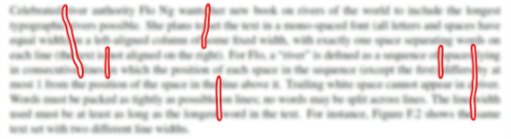
\includegraphics[width=10cm]{images/image1.png}
\end{center}

Ahora veamos la razón de mantener dos copias del grafo, la arista que tiene una longitud $10$ se considera dos veces. Durante la ejecución del algoritmo, primero se eliminará de la copia más pequeña del grafo, es decir, $G_S$ (mientras se recorre desde la longitud $200$ a $10$), y luego se eliminará de la copia más grande del grafo, es decir, $G_L$ (mientras se recorre para la longitud $8$ a $10$).

\nl

Como la eliminación puede ser costosa o puede tener una complejidad lineal, podemos mantener contadores que indicarán el rango en el que se debe considerar la lista de aristas. La complejidad temporal del enfoque anterior será $O(E * \log{E} + E * \log{V})$, $O(E \log{E})$ aparecerá debido a la lista de aristas de clasificación, y $O(E * \log{V})$ debido a Dijkstra.

\nl

\textbf{Código:} \href{https://gist.github.com/leynier/7b71cb4c6bf7f21e69f444bc60cad478}{gist.github.com/leynier/7b71cb4c6bf7f21e69f444bc60cad478}

\nl

\textbf{Fuente:} \href{https://www.codechef.com/problems/SPSHORT}{www.codechef.com/problems/SPSHORT}

\newpage

\nocite{*}
\bibliographystyle{unsrt}
\bibliography{dijkstra}

\end{document}
